\begin{figure}[t]
  \centering
  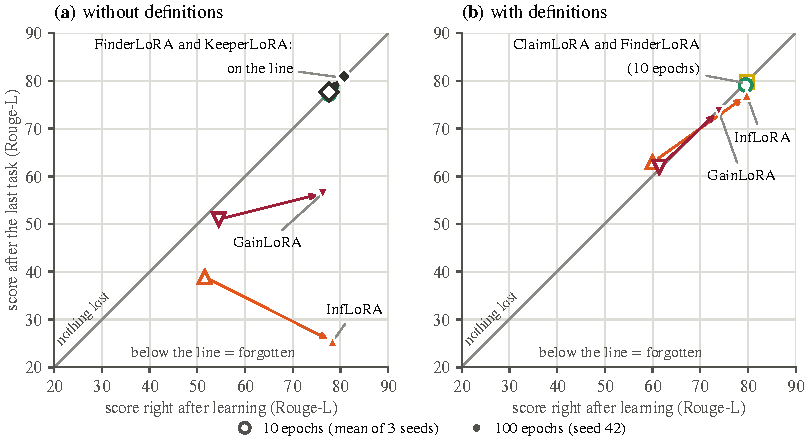
\includegraphics[width=\linewidth]{figures/learn_keep}
  \caption{Learned against kept, five tasks. A point is a method: its mean score right after
  learning ($x$) and after the last task ($y$). On the diagonal nothing is lost; the distance below
  it is what was forgotten. Hollow: 10 epochs (mean of three seeds); filled: \AudFullEpochs{} epochs
  (seed 42); an arrow goes from 10 to \AudFullEpochs{} epochs. (a)~Without definitions the two
  published methods learn more with more epochs and fall further below the diagonal; \recog{} and
  \handicap{} stay on it. (b)~With definitions the published methods stay near the diagonal (the
  control run); for our rules with definitions only 10-epoch runs exist.}
  \label{fig:learnkeep}
\end{figure}
